{\let\cleardoublepage\relax \chapter{Przyswajanie wiedzy}}

Hermann Ebbinghaus\cite{HumanMemory} (1850-1909) był Niemieckim psychologiem, który jako jeden z pierwszych zajmował się tematyką eksperymentalnej psychologii związanej z przyswajaniem wiedzy. 
Jednym z jego pierwszych eksperymentów było stworzenie testu, podczas którego uczył się zestawu 20 sylab, które były bezsensowne ze względu na fakt, iż w jego języku nie występowały żadne słowa, które ich używały.
Eksperyment ten pozwolił mu skonstruować pierwszą na świecie krzywą zapominania. Miała ona charakter eksponencjalny.  Możemy z niej wywnioskować, iż podczas początkowego okresu zapominania tracimy najwięcej zapamiętanych informacji.

\begin{figure}[h]
	\centering
	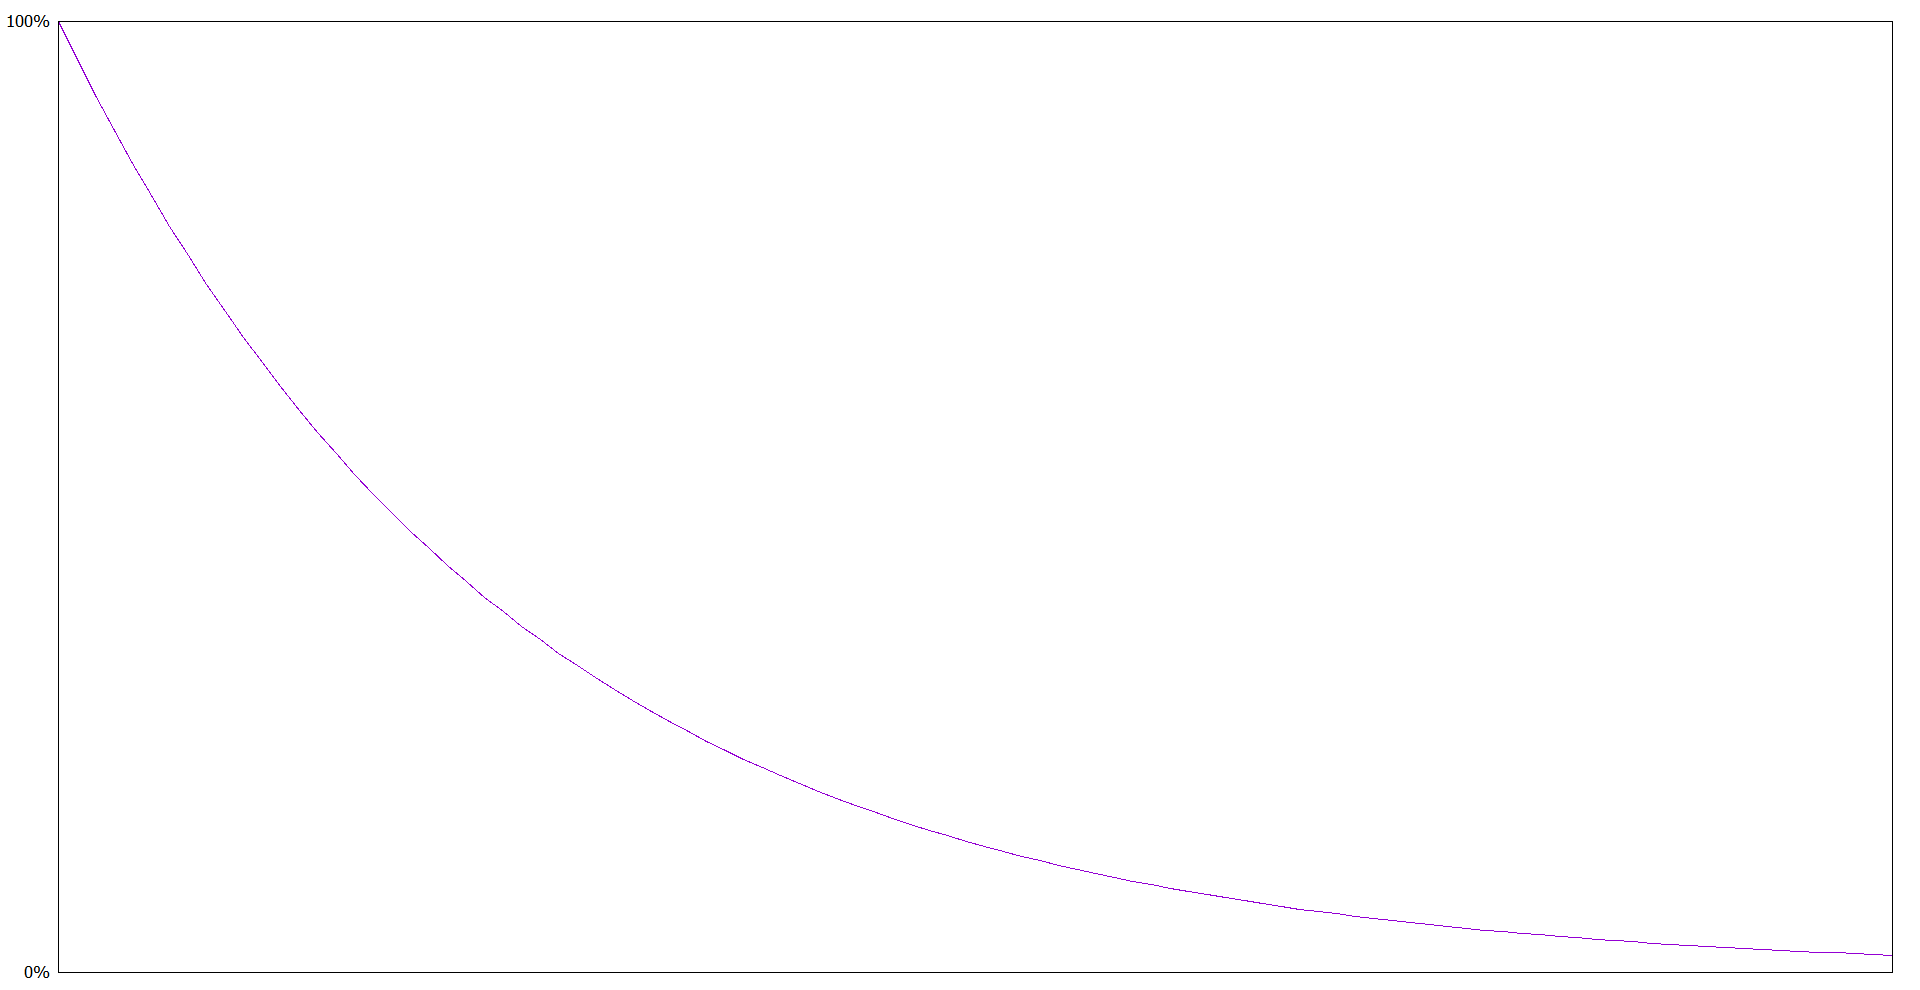
\includegraphics[width=\textwidth]{images/curve.png}
	 \caption{Eksponencjalna krzywa zapominania.}
\end{figure}

Trzeba także zwrócić uwagę na fakt, iż w rzeczywistości\cite{ForgettingCurve} mózg nie jest w stanie przyswoić danych informacji w 100\% po zakończeniu nauki. 

\section{Interwały potwórzeń}

W celu jak najlepszego zapamiętania wyuczonych informacji należy, poza odpowiednim programem nauczania, zwrócić uwagę na fakt, w jakich interwałach czasowych powtarzany jest przerabiany materiał\cite{ForgettingCurve}.
Interwał musi być wystarczająco krótki, aby zapobiec zapominaniu i wystarczająco długi, aby zbyt często nie przyswajać powtarzanego materiału.

\section{Efekt przewagi obrazów}

Efekt przewagi obrazów odnosi się do zjawiska, w którym zdjęcia i obrazy mają większą szanse na bycie zapamiętanymi niż ich zapisane odpowiedniki. 

Istnieje wiele badań \cite{PicturesRocks}\cite{SuperPictures}, które ukazują pozytywny wpływ obrazków na łatwość zapamiętania informacji. 

Istnieją także badania, które zjawisko pokazują w zupełnie innym świetle, pokazując brak pozytywnego wpływu obrazków na nauczanie języków obcych\cite{OverConfidence}.
\\
Wewnątrz projektu starano się wykorzystać powyższy efekt wymagając na użytkowniku zapamiętania, a następnie przypomnienia słowa w języku obcym wykorzystując do tego celu obrazki. Takie postępowanie w najgorszym wypadku będzie na równi efektywne z tradycyjnym.







{\let\cleardoublepage\relax \chapter{.NET}}


%https://docs.microsoft.com/en-us/dotnet/standard/tour
.NET jest platformą programistyczną umożliwiającą pisanie nowoczesnych aplikacji w językach wysokiego poziomu, do których zalicza się m.in C\#, VB oraz F\#. Platforma ta wyróżnia się tym iż:
\begin{itemize}
	\item Pozwala na użycie wielu języków programowania podczas pisania naszych programów.
	\item Ma zaimplementowane mechanizmy do obsługi operacji asynchronicznych i współbieżnych.
	\item Można ją stosować na różnych platformach, które posiadają środowisko wykonywalne .NET.
\end{itemize}
Wszystkie języki używane w platformie .NET kompilowane są do Wspólnego Języka Pośredniego (po ang. \textit{Common Intermediate Language}), który następnie jest tłumaczony na kod bajtowy i wykonywany za pomocą środowiska wykonywalnego danej implementacji .NET.

\begin{lstlisting}[frame=single, numbers=none,captionpos=b, 
caption={Przykładowy kod aplikacji "Hello World" w języku CIL}]
.assembly HelloWorld
.class auto ansi HelloWorldApp
{
     .method public hidebysig static void Main() cil managed
     {
          .entrypoint
          .maxstack 1
          ldstr "Hello world."
          call void [mscorlib]System.Console::WriteLine(string)
          ret
     }
}
\end{lstlisting}

%https://docs.microsoft.com/en-us/dotnet/standard/tour
% CLI ECMA http://www.ecma-international.org/publications/files/ECMA-ST/ECMA-335.pdf

\section{Implementacje .NET}

Każda aplikacja .NET jest uruchamiana na jednej z implementacji .NET. \\
Od roku 2016 wprowadzono .NET Standard - wspólny zestaw API, które każda z implementacji musi posiadać. Pozwala to na pisanie i używanie bibliotek programistycznych w różnych środowiskach .NET.

Istnieją aktualnie 4 główne implementacje .NET:

%https://docs.microsoft.com/en-us/dotnet/standard/components
\subsection{.NET Core}
Został napisany z myślą o tworzeniu aplikacji cross-platformowych, które mogą zostać uruchomione na serwerach, jak i środowiskach chmurowych. Potrafi działać na platformie Windows, macOS oraz Linux. Jest to pierwsza implementacja .NET, która została zaprojektowana przez Microsoft z myślą o wieloplatformowości.

%https://docs.microsoft.com/en-us/dotnet/framework/get-started/overview
\subsection{.NET Framework}
Pierwsza, oryginalna implementacja .NET, która istnieje od roku 2002. Składa się ze środowiska uruchomieniowego Common Language Runtime (CLR) oraz biblioteki standardowej zwanej jako Framework Class Library (FCL). CLR zapewnia aplikacjom wirtualną maszynę, na której wykonywany jest kod bajtowy skompilowany z języka CIL. Ta implementacja jest używana w tej pracy inżynierskiej.

%http://www.mono-project.com/docs/about-mono/
\subsection{Mono}
Darmowy projekt open-source prowadzony przez firmę Xamarin. Powodem stworzenia tego produktu była możliwość uruchamiania aplikacji napisanych w językach .NET na wielu platformach, jak i dostarczenie użytkownikom Linuxa narzędzi pozwalających na pisanie aplikacji w rodzinie języków .NET.
%https://docs.microsoft.com/en-us/windows/uwp/get-started/whats-a-uwp
\subsection{Universal Windows Platform (\textit{UWP})}
Implementacja, która umożliwia tworzenie aplikacji dla wszystkich platform używających Windows 10, Xboxa , niektórych urządzeń stworzonych przez Microsoft i dostosowanych urządzeń IoT.


\section{C\#}

C\# jest językiem programowania trzeciej generacji. Został opublikowany w roku 2001 przez firmę Microsoft. Jest on silnie typowanym językiem wielo-paradygmatowym umożliwiającym programowanie imperatywne, deklaratywne, generyczne, funkcjonalne, komponentowe i zorientowane obiektowo. Najnowszy jego standard został wydany w listopadzie 2017 roku i jest oznaczony jako wersja 7.2. Wchodzi on w grupę języków .NET przez co jest kompilowalny do języka CIL. \cite{CPlotekInfo}
\begin{minipage}{\linewidth}
\begin{lstlisting}[frame=single, numbers=none,captionpos=b, 
caption={Przykładowy kod aplikacji "Hello World" w języku CIL}]
using System;
namespace HelloWorld
{
    class Hello 
    {
        static void Main() 
        {
            Console.WriteLine("Hello World!");
            Console.ReadKey();
        }
    }
}
\end{lstlisting}
\end{minipage}
\newpage
{\let\cleardoublepage\relax \chapter{ASP.NET MVC}}

%https://msdn.microsoft.com/en-us/library/dd381412(v=vs.108).aspx

ASP.NET MVC jest frameworkiem do budowania aplikacji internetowych w oparciu o wzorzec architektoniczny Model-View-Controller (MVC). Wykorzystuje implementacje .NET Framework do uruchamiania skompilowanego kodu źródłowego.


\section{Model-Widok-Kontroler}

Większość dzisiejszych systemów komputerowych działa na zasadzie wyświetlania danych, które aktualnie znajdują się w bazie danych i ewentualnie ich modyfikacji. W celu ujednolicenia tych systemów stosowany jest wzorzec Model-Widok-Kontroler(ang. Model-View-Controller), który rozdziela logikę aplikacji na 3 główne segmenty:
\begin{enumerate}
	\item Model - Służy do pobierania, przechowywania i zamiany danych.
	\item Kontroler - przetwarza zapytania użytkownika.
	\item Widok - Służy do wyświetlania informacji .
\end{enumerate}

% Framework do budowania stron internetowych w oparciu o technologie .NET
\begin{figure}[h]
	\centering
	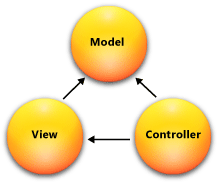
\includegraphics[height=50.5mm]{images/mvc.png}
	 \caption{Model MVC. Źródło: msdn.microsoft.com}
\end{figure}

Cała aplikacja została skonstruowana zgodnie z tym wzorcem projektowym. ASP.NET MVC posiada wiele narzędzi, które ułatwiają zastosowanie tego wzorca. Dostarczana jest klasa bazowa \textbf{Controller}, która posiada wszystkie podstawowe metody do wyświetlania odpowiednich treści danych i zarządzania zapytaniami.

Wzorzec MVC niesie za sobą korzyści związane z warstwą wyświetlania danych. Jest to warstwa aplikacji, w której bardzo często dochodzi do zmian. Dzięki odseparowaniu danych od widoku jesteśmy w stanie tworzyć, jak i zmieniać widoki, bez wpływu na kod biznesowy aplikacji.

\section{Wzorzec Repozytorium}

Wewnątrz aplikacji używana będzie baza danych Microsoft SQL. Do komunikacji z bazą bardzo często jest tworzony kod, który zwraca podobne dane. W celu zmniejszenia redundancji kodu, jak i odseparowania zależności i odpowiedzialności wykorzystany został wzorzec Repozytorium (z ang. Repository Pattern)\cite{RepositoryUnitOfWorkPattern}.

Wzorzec ten wykorzystuje obiekty, zwane repozytoriami, których zadaniem jest pobieranie i modyfikowanie danych po stronie serwera SQL. Nie zawierają żadnej logiki biznesowej i są niezwiązane z resztą kodu danej aplikacji. 

\begin{figure}[h]
	\centering
	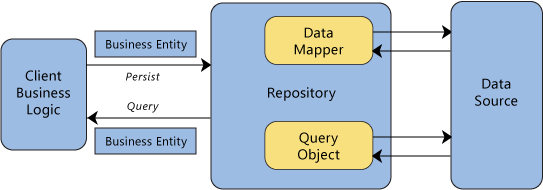
\includegraphics[width=\textwidth]{images/RepositoryPattern.png}
	 \caption{Wzorzec repozytorium. Źródło: msdn.microsoft.com}
\end{figure}

Wewnątrz projektu cały wzorzec repozytorium został oparty na interfejsach \textbf{IRepository} i \textbf{IRepository<T>} (który implementuje \textbf{IRepository}). W założeniu te interfejsy definiują operacje, które można zrealizować na danym obiekcie klasy 'T'. Informacja o sposobie realizacji operacji jest zdefiniowana w klasie \textbf{RepositoryBase<T>}.
Wszystkie kolejne stworzone repozytoria dziedziczą po \textbf{RepositoryBase<T>} a ich interfejsy implementują \textbf{IRepository<T>}. 
Takie działanie pozwala nam na separację reprezentacji persystentnej (baza danych) i reprezentacji bieżącej (repozytoria). Wystarczy, iż zmienimy \textbf{RepositoryBase<T>} na jakąkolwiek inną klasę implementującą \textbf{IRepository<T>}. Dzięki temu możemy zastąpić Microsoft SQL inną implementacją.


\begin{figure}[h]
	\centering
	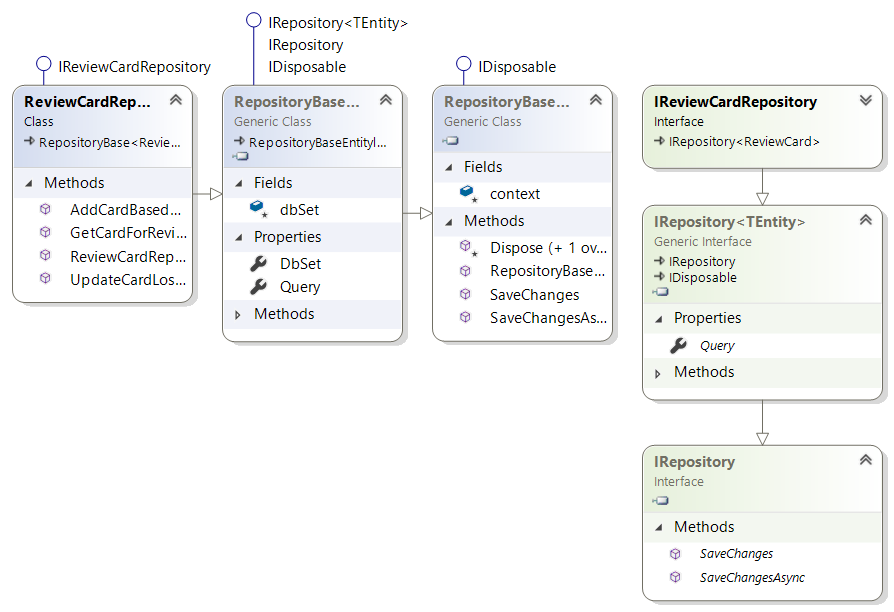
\includegraphics[width=\textwidth]{images/ReviewRepository.png}
	 \caption{Repozytorium ReviewCardRepository wraz z implementowanymi interfejsami i odziedziczonymi klasami.}
\end{figure}

\section{Jednostka Pracy}
%https://docs.microsoft.com/en-us/aspnet/mvc/overview/older-versions/getting-started-with-ef-5-using-mvc-4/implementing-the-repository-and-unit-of-work-patterns-in-an-asp-net-mvc-application

Wzorzec Jednostki Pracy (z ang. Unit of Work)\cite{RepositoryUnitOfWorkPattern} ma na celu uporządkowanie pracy z repozytoriami za pomocą umieszczenia ich wszystkich w jednej klasie. Dodatkowo dzięki temu rozwiązaniu wszystkie repozytoria współdzielą kontekst dostępu do bazy Microsoft SQL. Zapisanie danych odbywa się poprzez wywołanie metody \textbf{SaveChanges} wewnątrz Jednostki Pracy (SaveChanges jest konwencją wewnątrz projektu).

\begin{figure}[h]
	\centering
	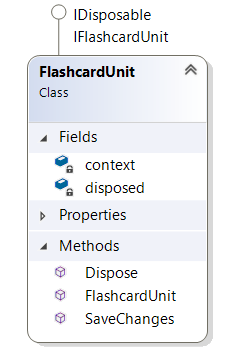
\includegraphics{images/UnitOfWork.png}
	 \caption{Jednostka pracy wykorzystywana w projekcie.}
\end{figure}
\newpage

\section{Mapowanie obiektowo-relacyjne}

Wewnątrz projektu zostało wykorzystane narzędzie Entity Framework pozwalająnce na korzystanie z mapowania obiektowo-relacyjnego. Dzięki tej technice można uprzednio zdefiniowane dane tabelaryczne odwzorować za pomocą klas, które zostaną stworzone na podstawie definicji tabel i relacji między nimi. Powstałe klasy są używane wewnątrz kolekcji, implementujących interfejs \textbf{IQueryable<T>}, na których możemy wykonywać zapytania z pomocą \textbf{LINQ}a, które następnie zostaną przetłumaczone na zapytania SQL.
\\ \\
Takowe rozwiązanie ma wiele zalet :
\begin{enumerate}
	\item Dane z danej tabeli można otrzymać zawsze w tym samym formacie.
	\item Zmniejsza to zakres potrzebnych umiejętności w celu pobrania danych. Dany programista nie musi znać języka SQL, aby w sposób bezproblemowy pobrać interesujące go dane, nawet gdy tworzy bardzo skomplikowane zapytania.
	\item Łatwiejsza nawigacja po zależnościach między tabelami. Na danym typie można wykorzystać operacje \textbf{Find All References}, która wskaże miejsca jego użycia w kodzie.
	\item Operacje na interfejsie \textbf{IQueryable<T>} pozwalają na pobranie danych dopiero, gdy będą nam potrzebne za pomocą techniki lazy loading.
\end{enumerate}

\section{Wstrzykiwanie zależności}

Wstrzykiwanie zależności (po ang. Dependency Injection) jest wzorcem projektowym, którego działanie polega na tym, iż obiekty aplikacji nie muszą tworzyć zależnych od siebie obiektów, lecz są tworzone przez obiekt nadrzędny dla użytku tych klas. 

Informacja o tym, jakie obiekty powinny zostać dostarczone danej instancji jest przekazywana najczęściej poprzez listę argumentów konstruktora bądź przy wywołaniu specjalnych metod.

Wewnątrz projektu w celu realizacji tego wzorca wykorzystana została biblioteka Ninject\cite{NinjectGithub}. Z pomocą dodatkowej biblioteki \textbf{Ninject.Web.Common} jest ona w stanie w łatwy sposób zintegrować się z aplikacją ASP.NET MVC wykorzystując interfejs \textbf{IDependencyResolver}. 

Każde utworzenie kontrolera wewnątrz aplikacji ASP.NET MVC wiąże się wpierw z odpytaniem aktualnie używanego IDependencyResolvera o próbę utworzenia takowego kontrolera. W tym miejscu zaczyna działać Ninject, który stara się utworzyć obiekt. Gdy konstruktor danej klasy będzie zawierał jakiekolwiek parametry to Ninject będzie starał się je utworzyć na podstawie zdefiniowanych uprzednio bindingów. Jeśli okaże się, że stworzenie obiektu kontrolera jest niemożliwe, to zwracany jest błąd wewnętrzny 500.
\\
Stworzenie bindingów, które będą informować, na jakich zasadach odbywa się tworzenie żądanych obiektów, jest wykonywane za pomocą metody \textbf{Bind} znajdującej się w Kernelu Ninjecta.

%\begin{lstlisting}[frame=single, numbers=none,captionpos=b, 
%caption={Przykładowy kod bindowania dla biblioteki Ninject}]
%public static void RegisterServices(IKernel kernel)
%{
%kernel.Bind<FlashcardsEntities>().ToSelf().InRequestScope();
%kernel.Bind<IFlashcardRepository>().To<FlashcardRepository>().InRequestScope();
%}
%\end{lstlisting}

\begin{figure}[h]
	\centering
	\includegraphics[width=\textwidth]{images/ninject.png}
	 \caption{Proces bindowania z wyszczególnionymi częściami składowymi.}
\end{figure}

Pierwsza część bidowania odpowiada za przekazanie informacji o tym jakiego \textbf{Providera} należy użyć w celu zwrócenia instancji danego typu.
Metody \textbf{ToSelf()} i \textbf{To<T>()} używają wbudowanego \textbf{StandardProvider}a. Pierwsza z metod zawsze będzie informowała o tym, iż należy zwrócić obiekt tego samego typu, gdzie druga konkretnie informuje jaki typ powinien zostać zwrócony w wyniku danego zapytania.

Ninject oferuje także opcje stworzenia własnych providerów. Można to osiągnąć za pomocą stworzenia klasy dziedziczącej po \textbf{Provider<T>} lub wykorzystania delegatów wewnątrz metody \textbf{ToMethod(Func<IConext, T>)}.

%https://github.com/ninject/ninject/wiki/Object-Scopes
Ninject w swoim domyślnym zachowaniu zawsze tworzy nowy obiekt danej klasy, gdy zostanie poproszony o instancje danego typu. Nie zawsze jest to jednak sytuacja pożądana. Każdy bind posiada możliwość zdefiniowana osobnego zasięgu w którym będzie on obowiązywał. Umożliwi to współkorzystanie z danego obiektu wewnątrz danego zakresu. W wypadku środowiska webowego bardzo często stosowanym zasięgiem jest \textbf{InRequestScope()}, które powoduje, iż obiekty danego typu stworzone przez Ninject są współdzielone w trakcie danego zapytania. 

Takie działanie niesie za sobą szereg korzyści. Nie tylko nie ponosimy kosztów tworzenia nowych obiektów, lecz także jesteśmy w stanie współdzielić dane informacje pomiędzy różnymi serwisami. (Np. repozytoria nie muszą wykonywać dodatkowych zapytań SQL, gdyż część wyników znajduje się ich w cache'u)

\newpage
{\let\cleardoublepage\relax \chapter{Microsoft SQL Server}}

Microsoft SQL Server\cite{SqlServer} jest aplikacją, umożliwiającą zarządzanie serwerami baz danych. Został stworzony przez firmę Microsoft. Jego pierwsza edycja ukazała się w roku 1989.

Do tworzenia zapytań wykorzystano tutaj język Transact-SQL (T-SQL). Jest to rozszerzenie języka SQL (Structured Query Language), które między innymi wprowadza:

\begin{enumerate}
	\item Lokalne zmienne.
	\item Blok \textbf{Try Catch}, wspierający obsługę wyjątków.
	\item Dodatkowe funkcjonalności związane z obsługą tekstu, kalendarza i matematyki.
	\item Możliwość tworzenia pętli oraz instrukcji warunkowych.
	\item Procedury, funkcje składowane i wyzwalacze.
\end{enumerate} 

W celu integracji serwera Microsoft SQL z projektem napisanym w języku C\# należy pobrać paczkę NuGet\footnote{NuGet jest menadżerem paczek w środowisku .NET.\cite{Nuget}} o nazwie \textbf{System.Data.SqlClient}.




\newpage
{\let\cleardoublepage\relax \chapter{Testy}}

%wykorzystuje tutaj metodę bottom-up

Aplikacje tworzone w dzisiejszych czasach wymagają dostarczenia zestawu testów, których zadaniem jest sprawdzenie poprawności działania aplikacji. Z tego też powodu napisany został zestaw testów, które sprawdzają, czy poszczególne komponenty aplikacji działają poprawnie.

\section{Testy Jednostkowe}

Testy jednostkowe mają za zadanie sprawdzić poprawność działania pojedynczego modułu. Wszelkie odwołania do innych komponentów zostają zastąpione przez atrapy obiektów (po ang. mock objects), które symulują działanie ich prawdziwych odpowiedników.
 Wewnątrz projektu do operacji związanych z atrapami wykorzystany został framework Moq, który zawiera także dodatkowe funkcjonalności pozwalające ocenić czy dany test przebiegł poprawnie.
Testy zostały ułożone zgodnie ze wzorcem AAA\cite{UnitTestingMicrosoft} - Aranżacja (po ang. Arrange) Akcja (po ang. Act) Asercja (po ang. assert).  Dzięki temu testy są konsystentne i czytelne, przez co nie potrzeba dużej ilości czasu w celu zaznajomienią się z nimi.

\begin{lstlisting}[frame=single, numbers=none,captionpos=b, 
caption={Przykładowy test jednostkowy wykorzystujący wzorzec AAA}]
public void StopLastTraining_assert_tests()
{
	//Aranżacja - stworzenie wewnętrznej atrapy obiektu dla atrapy serwisu
	mockTraining();
	//Akcja
	trainingReviewService.StopLastTraining();
	//Asercja - sprawdzenie poprawności wykonania
	trainingRepository.Verify(x => x.Remove(It.IsAny<long>()), Times.Once);
	unit.Verify(x => x.SaveChanges(), Times.Once); //wykorzystanie funkcjonalności frameworku Moq w celu sprawdzenia czy dana metoda została wywołana.
	Assert.AreEqual(null, sessionService.Object.UserInfo.TrainingInfo);
}
\end{lstlisting}

\section{Testy Integracyjne}

Testy integracyjne mają za zadanie pokazać poprawną komunikacje pomiędzy modułami w projekcie. Modułem może być każdy komponent zaprogramowany na potrzeby projektu jak i zewnętrzny system (np. system obsługi plików). Wszystkie moduły, które nie są testowane w danym teście powinny zostać zastąpione przez odpowiednie atrapy.

\begin{lstlisting}[frame=single, numbers=none,captionpos=b, 
caption={Test integracyjny wykorzystany w projekcie.}]
[TestMethod]
public void ExistTest()
{
	using (var temp = new WindowsTempFile())
		Assert.IsTrue(File.Exists(temp.Path));
}}
\end{lstlisting}

\newpage
{\let\cleardoublepage\relax \chapter{Kaskadowe Arkusze Styli}}

Kaskadowe Arkusze Styli (po ang. Cascading Style Sheets, w skrócie CSS)\cite{CSSDoc} wykorzystywane są w celu opisu sposobu wyświetlania elementów stron WWW. Pozwalają zdefiniować między innymi takie właściwości elementów jak: kolory, czcionki, położenie. Dzięki oddzieleniu warstwy danych od warstwy prezentacji możliwe jest wykorzystanie tych samych arkuszów styli na wielu stronach. 
W celu określenia wyglądu danego elementu należy zdefiniować odpowiednią regułę, na którą składa się :
\begin{enumerate}
	\item Selektor, który określa dla jakich elementów przeznaczona jest dana reguła.
	\item Zestaw właściwości wraz z przypisanymi do nich wartościami
\end{enumerate}

\begin{lstlisting}[frame=single, numbers=none,captionpos=b, 
caption={Przykład prostej reguły, dzięki której wszystkie paragrafy będą miały domyślnie kolor pomarańczowy.}]
p //seletor p
{
//Właściwość color do której przypisano wartość orange
    color: orange;
}
\end{lstlisting}

\section{Syntaktycznie Zarąbiste Arkusze Styli}

W dzisiejszym świecie nikt obeznany z technologią tworzenia stron internetowych nie używa już czystego języka CSS do tworzenia arkuszy styli. 
Wynika to z faktu występowania zbyt dużej redundancji kodu, która jest związana z tym, iż niektóre fragmenty strony są formatowane zawsze w ten sam sposób (np. motyw kolorystyczny dla większości elementów jest ten sam). 

Jest to spowodowane brakiem zmiennych, szablonów, oraz innych konstrukcji, które pomogłoby w ograniczeniu powyższego problemu. 

Z tego też powodu powstały rozwiązania niedogodności występujących w języku CSS. Jednym z nich jest język SASS - Syntactically Awesome Style Sheets (z ang. Syntaktycznie Zarąbiste Arkusze Styli)\cite{Sass}. Jest on kompatybilny ze wszystkimi wersjami CSS, przez co każdy kod napisany w CSS jest z nim zgodny. Oferuje bardzo dużo funkcjonalności, między innymi:
\begin{enumerate}
	\item Zmienne, które pozwalają wielokrotnie używać danych wartości
	\item Możliwość zagnieżdżania reguł w innych regułach.
	\item Możliwość załączania plików pozwalająca na podział arkuszy styli.
	\item Mixin - szablony reguł, które można ponownie wykorzystywać.
	\item Dziedziczenie reguł za pomocą słówka kluczowego \textbf{@extend}
	\item Za pomocą operatorów \textbf{+}, \textbf{-}, \textbf{*}, \textbf{/}, \textbf{\%} można wykonywać operacjach na liczbach.
\end{enumerate}


\begin{lstlisting}[frame=single, numbers=none,captionpos=b, 
caption={Przykładowy kod SCSS wykorzystujący mixin.}]
@mixin border-radius($radius) {
  -webkit-border-radius: $radius;
     -moz-border-radius: $radius;
      -ms-border-radius: $radius;
          border-radius: $radius;
}

.box { @include border-radius(10px); }
\end{lstlisting}

\newpage
{\let\cleardoublepage\relax \chapter{Scala}}

Scala\cite{ScalaWiki} jest językiem programowania ogólnego zastosowania, który został wprowadzony na rynek przez Laboratorium "École Polytechnique Fédérale de Lausanne". Jest to język kompilowalny bezpośrednio do kodu bajtowego Javy, przez co programy w nim napisane z łatwością uruchamiają się w środowisku wykonywalnym maszyny wirtualnej Javy. 
Scala jest językiem wielo-paradygmatowym\cite{ScalaTour}. Korzysta z dobrodziejstw programowania funkcjonalnego i obiektowego.

\begin{lstlisting}[frame=single, numbers=none,captionpos=b, 
caption={Hello world napisany w języku Scala.}]
object HelloWorld {
  def main(args: Array[String]): Unit = {
    println("Hello, world!")
  }
}
\end{lstlisting}

\section{Javascript}

Javascript jest głównym językiem programowania wykorzystywanym na stronach internetowych. Może być on interpretowany bądź kompilowany metodą Just In Time, która kompiluje kod tuż przed jego wykonaniem. Jest to dynamiczny język wieloparadygmatowy bazujący na prototypach. Wspiera programowanie obiektowe, imperatywne i deklaratywne.\cite{AboutJS}
Javascript jako język posiada wiele problemów, które mogą doprowadzić do wystąpięnia błędów, między innymi takich jak:
\begin{enumerate}
	\item Niejawne rzutowania, które objawiają się przy użyciu operatora ==. Są przyczyną wielu trudnych do odkrycia błędów
	\item Automatyczne wstawianie średników, co może spowodować, iż program działa inaczej niż zamierzał to programista. Czasami potrafi to uratować program napisany przez programistę, lecz często prowadzi do dziwnych i niezrozumiałych błędów, takich jak w przypadku poniższego listingu: \ref{lst:javascriptSUCKS}
	\item Niezrozumiałe zachowana różnych funkcji. Metoda sortująca domyślnie sortuje tablice liczb w porządku alfabetycznym nie zwracając uwagi na fakt, iż w tablicy nie występuje ani jeden ciąg znakowy.
	\item Zmienne, które w każdej chwili mogą zmienić swój typ. Pomimo tego, iż jest to błąd programistyczny to w wyniku tej niedogodności powstają trudne do namierzenia błędy w kodzie.
\end{enumerate}

\begin{lstlisting}[label={lst:javascriptSUCKS},
frame=single, numbers=none,captionpos=b, 
caption={Przykład niepoprawnego kodu Javascript wynikłego z automatycznego wstawienia średnika}]
function foo() {
    return // Tutaj zostanie wstawiony średnik.
        {
            bar : "test"
        };
}
\end{lstlisting}


Z tego też powodu powstały języki, które starają się być lepsze i przyjaźniejsze dla programisty niż Javascript. Jest to między innymi: Typescript, Coffescript, Dart czy Scala.js. Takie języki programowania nie są wykonywane/kompilowane bezpośrednio w przeglądarce, lecz wpierw są kompilowane do kodu Javascript. Spowodowane jest to używaniem przez przeglądarki jedynie języka Javascript do wykonywania kodu\footnote{Wyjątkiem jest tutaj przeglądarka Dartium, która posiada maszynę wirtualną języka Dart\cite{Dartium}}. 

\begin{figure}[h]
	\centering
	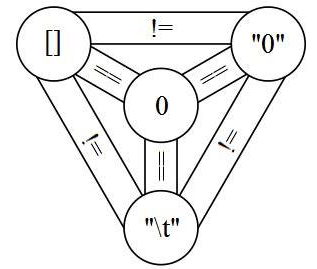
\includegraphics{images/javagod.png}
	 \caption{Przykład dziwnego zachowania języka Javascript. Źródło: devrant.com}
\end{figure}

\section{Scala w wersji JS}

Scala.js jest narzędziem umożliwiającym kompilacje kodu Scali do języka Javascript. Umożliwia to pozbycie się niedogodności wymienionych powyżej. Jest to możliwe dzięki:



\begin{enumerate}
	\item Silnemu typowaniu, dzięki któremu pisany kod nie zawiera bardzo prostych błędów.
	\item Nie skupianiu się na dziwnych i frustrujących \hyperref[lst:javascriptSUCKS]{aspektach języka Javascript}.
	\item Środowiskom programistycznym wspierającym pracę programisty przez podpowiadanie składni, łatwą nawigację po kodzie źródłowym oraz inne udogodnienia.
	\item Możliwości wykrycia błędów w trakcie kompilowania kodu źródłowego.
\end{enumerate}


\subsection{sbt}
	

sbt (Simple Build Tool) jest narzędziem o otwartym kodzie źródłowym, pozwalającym na zarządzanie procesem budowania aplikacji napisanej w języku Scala lub Java. Jest to narzędzie bardzo rozbudowane, które m.in. umożliwia:
\begin{enumerate}
	\item Współpracę z wieloma narzędziami testującymi dla scali.
	\item Inkrementacyjne kompilowanie i testowanie.
	\item Zarządzanie zależnościami przy pomocy menadżera paczek Ivy.\cite{ApacheIvy}
	\item Ciągłe wdrażanie, kompilowanie i testowanie kodu.
\end{enumerate}



%Scala jest zorientowana obiektowo ze względu na to, iż każda zmienna jest obiektem. Mamy do wykorzystania klasy i cechy (ang. traits), wraz z mechanizmami dziedziczenia. Pozwala to odwzorować 

\subsection{Proces budowania projektu}

Proces kompilacji projektu jest podzielony na 3 etapy\cite{HandsOnScalaPipeline}:
\begin{enumerate}
	\item Początkową kompilację
	\item Szybką optymalizację
	\item Pełną optymalizację (Opcjonalny)
\end{enumerate}

\subsubsection{Początkowa kompilacja}

W trakcie kompilacji pliki .scala są kompilowane do plików .class i .sjsir. 
Pliki .class nie biorą udziału w tworzeniu kodu javascript. Ich zadaniem jest współpraca z innymi narzędziami, które być może będą ich używać. Przykładem takiego narzędzia może być \textbf{IntelliJ} lub \textbf{Eclipse}, które plików .class używają w celu wspomagania programisty w trakcie pisania kodu.
Pliki .sjsir (Nazwa rozszerzenia jest skrótem od ,,ScalaJS Intermediate Representation'')\cite{ScalaCompilationProcess} zawierają kod przejściowy między Scalą a Javascriptem. Większość konstrukcji została zastąpiona przez ekwiwalenty z języka Javascript. 
Gdybyśmy połączyli wszystkie pliki .sjsir, wyprodukowane przez sbt to ich wynikiem byłby plik większy niż 20 MB. Wynika to z faktu, iż w tym pliku nadal znajduje się wiele niepotrzebnych bibliotek i konstrukcji. Jak na przykład \textbf{cała} biblioteka standardowa Scali.

\begin{minipage}{\linewidth}
\begin{lstlisting}[label={lst:scalasbt},
frame=single, numbers=none,captionpos=b, 
caption={Przykładowy plik .sjsir dla projektu wyświetlającego HelloWorld na ekranie.}]
module class Ltutorial_webapp_TutorialApp$ extends O {
  def main__AT__V(args: T[]) {
    this.appendPar__Lorg_scalajs_dom_raw_Node__T__V
    (mod:Lorg_scalajs_dom_package$.document__Lorg_scalajs_dom_raw_HTMLDocument
    ()["body"], "Hello World")
  }
  def appendPar__Lorg_scalajs_dom_raw_Node__T__V(targetNode: any, text: T) {
    val parNode: any = mod:Lorg_scalajs_dom_package$.document__Lorg_scalajs_dom_raw_HTMLDocument()
    ["createElement"]("p");
    val textNode: any = mod:Lorg_scalajs_dom_package$.document__Lorg_scalajs_dom_raw_HTMLDocument()
    ["createTextNode"](text);
    parNode["appendChild"](textNode);
    targetNode["appendChild"](parNode)
  }
  def init___() {
    this.O::init___();
    mod:Ltutorial_webapp_TutorialApp$<-this
  }
}
\end{lstlisting}
\end{minipage}
\subsubsection{Szybka optymalizacja}

W celu optymalizacji poprzedniego kroku stosuje się szybką optymalizację kodu .sjsir, która jako rezultat swej pracy stworzy kod Javascript. W tym celu należy użyć optymalizatora FastOptJS poprzez wpisanie komendy \textbf{FastOptJS} w sbt. Optymalizacja ma na celu:
\begin{enumerate}
	\item Wyeliminowanie fragmentów kodu, które są nieużywane. Na przykład kod biblioteki standardowej, który nie zostanie wywołany.
	\item Inline'owanie małych funkcji. Zmniejsza to koszt wywołań i wielkość kodu.
	\item Zmiana zmiennych na stałe, jeśli ich wartość jest znana w trakcie kompilacji.
\end{enumerate}

Dzięki tej operacji kod wykonywalny zmniejszy się z 20 MB do 1.5-2.5MB\cite{ScalaCompilationProcess}.


\subsubsection{Pełna optymalizacja}

Kod, który jest tworzony przez Scala.js jest zgodny z restrykcjami narzuconymi przez kompilator Closure\cite{Closure}. Jest to narzędzie stworzone przez firmę Google, które potrafi optymalizować kod Javascript.\cite{ClosureCompiler} Celem tego kroku jest zmniejszenie rozmiaru pliku Javascript i uczynienie konstrukcji w nim występujących bardziej wydajnymi.
W wyniku tego procesu otrzymywany jest plik wykonywalny o rozmiarze między 150KB do kilkuset KB\cite{ScalaCompilationProcess}.
W celu użycia pełnej optymalizacji należy wywołać polecenie \textbf{FullOptJS} w sbt.

\subsubsection{Pliki javascript}

W wyniku działań optymalizatorów tworzone są poniższe pliki javascript. Należy mieć na uwadze fakt, iż pliki bibliotek muszą zostać dołączone do kodu strony przed plikiem z kodem wykonywalnym.

\begin{center}
\begin{tabular}{| l | l | p{6cm} |}
\hline
Typ kompilacji & Wytworzony plik & Zawartość pliku \\ \Xhline{3\arrayrulewidth}

FastOptJS & scala-js-[Nazwa-Projektu]-fastopt.js & Plik z kodem wykonywalnym \\ \hline

FastOptJS & scala-js-[Nazwa-Projektu]-fastopt.js.map & Plik mapujący kod Javascript do kodu Scali. \\ \hline

FastOptJS & scala-js-[Nazwa-Projektu]-jsdeps.js & Plik z kodem zewnętrznych bibliotek użytych w procesie tworzenia aplikacji \\ \hline

 \Xhline{2\arrayrulewidth}

FullOptJS & scala-js-[Nazwa-Projektu]-opt.js & Plik z kodem wykonywalnym \\ \hline

FullOptJS & scala-js-[Nazwa-Projektu]-opt.js.map & Plik mapujący kod Javascript do kodu Scali. \\ \hline

FullOptJS & scala-js-[Nazwa-Projektu]-jsdeps.min.js & Plik z kodem zewnętrznych bibliotek użytych w procesie tworzenia aplikacji. \\ \hline
\end{tabular}
\end{center}
\subsubsection{Debugowanie}


Jednym z najważniejszych procesów, które na celu mają znalezienie błędów w powstałym kodzie jest debugowanie. Proces debugowania aplikacji powinien umożliwiać programiście przynajmniej możliwość zatrzymania kodu w dowolnym miejscu, podejrzenia kodu źródłowego jak i możliwość odczytu i modyfikacji zmiennych.

Kod stworzony za pomocą kompilatora scala.js jest bardzo łatwy w debugowaniu. Przeglądarki posiadają możliwość dołączenia mapy kodów źródłowych, które do danych linijek kodu javascript przypisują ich odpowiedniki w pliku źródłowym. Umożliwia to prace z oryginalnym kodem źródłowym podczas używania przeglądarki internetowej. 

Pliki z mapami źródłowymi mają format \textbf{\{SkompilowanyPlik\}.map}, gdzie SkompilowanyPlik jest artefaktem naszego procesu kompilacji, np.  \textbf{scala-js-[Nazwa-Projektu]-fastopt.js}. 
\afterpage{
\begin{figure}[h]
\begin{center}
	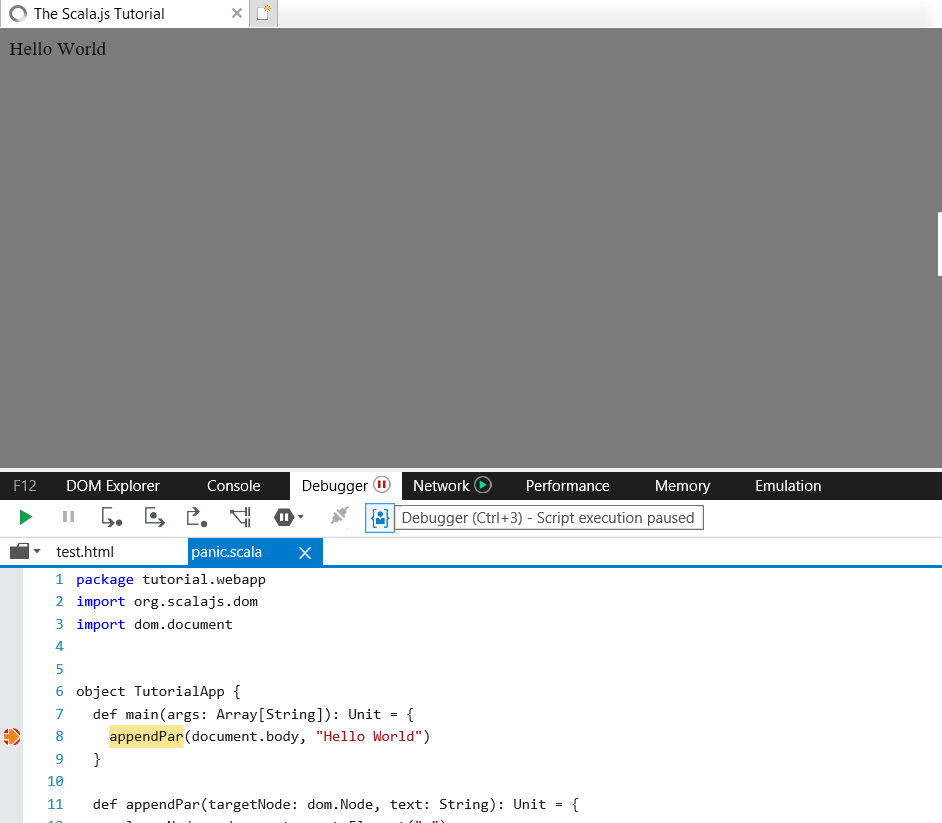
\includegraphics[width=\textwidth]{images/debug.png}
	 \caption[Przykład procesu debugowania kodu. Nasz program zostaje zatrzymany na linijce przed dodaniem napisu Hello World.]
	 {Przykład procesu debugowania kodu. Program zostaje zatrzymany na linijce przed dodaniem napisu Hello World. \footnotemark}
	 \end{center}
\end{figure}
\footnotetext{Na obrazku na stronie widnieje już napis Hello World. Jest to artefakt, który został stworzony przy poprzednim uruchomieniu strony i jeszcze się nie odświeżył.}

}


\newpage

\subsection{Hello World}

Za pomocą powyższych metod i narzędzi można stworzyć w bardzo prosty sposób przykładową aplikację wykorzystującą język Scala.js. W tym celu należy użyć polecenia \textbf{sbt new sbt/scala-seed.g8}, które spowoduje utworzenie minimalnego projektu Scali. Aby projekt wykorzystywał Scale.js należy w nim wykonać parę zmian:


\begin{enumerate}
	\item Należy dodać plik ./project/plugins.sbt\footnote{./ jest katalogiem głównym projektu w tym przypadku.}, wewnątrz którego znajdzie się instrukcja \textbf{addSbtPlugin("org.scala-js" \% "sbt-scalajs" \% "0.6.20")}, która poinformuje sbt o konieczności użycia pluginu Scali.js.
	\item W pliku ./project/build.properties musi zostać określona wersja narzędzia sbt, którym będzie kompilowany projekt.
	\item Plik build.sbt, który zawiera ustawienia związane z budową projektu, musi zostać zmodyfikowany w celu użycia plugina Scali.js jak i pomocniczych bibliotek. Przykładowy plik, który jest używany w projekcie można zobaczyć na listingu \ref{lst:scalasbt}.
\end{enumerate}

Po takim zabiegu należy już tylko dodać kod źródłowy Scali do folderu ./src/main/scala. Przykładowy kod można znaleźć na listingu \ref{lst:helloscalajs}

\begin{minipage}{\linewidth}
\begin{lstlisting}[label={lst:scalasbt},
frame=single, numbers=none,captionpos=b, 
caption={Plik .sbt, który jest wykorzystywany w projekcie.}]
enablePlugins(ScalaJSPlugin)
libraryDependencies += "org.scala-js" %%% "scalajs-dom" % "0.9.1"
libraryDependencies += "be.doeraene" %%% "scalajs-jquery" % "0.9.1"

name := "Flashcards"
scalaVersion := "2.12.2"

// Informacja o tym, iż chcemy aby nasz kod zawsze miał uruchamianą metodę main po wczytaniu witryny.
scalaJSUseMainModuleInitializer := true

skip in packageJSDependencies := false
jsDependencies += "org.webjars" % "jquery" % "2.1.4" / "2.1.4/jquery.js" 
jsDependencies += "org.webjars.bower" % "jsrender" % "1.0.0-rc.70" / "1.0.0-rc.70/jsrender.js"
\end{lstlisting}
\end{minipage}

\begin{minipage}{\linewidth}
\begin{lstlisting}[label={lst:helloscalajs},
frame=single, numbers=none,captionpos=b, 
caption={Przykładowy projekt w Scali.js wypisujący napis Hello World na stronie.}]
package helloworld
import org.scalajs.dom
import dom.document

object TutorialApp {
  def main(args: Array[String]): Unit = {
    appendPar(document.body, "Hello World")
  }

  def appendPar(targetNode: dom.Node, text: String): Unit = {
    val parNode = document.createElement("p")
    val textNode = document.createTextNode(text)
    parNode.appendChild(textNode)
    targetNode.appendChild(parNode)
  }
}
\end{lstlisting}
\end{minipage}
